If it is necessary to move this selection to a front panel switch, this can be accomplished simply by attaching a
\acronym{DPDT} switch to each jumper block header like this:
%  o
%  o      o<-o  o
%  o      o<-o  o
%  o
\begin{center}
	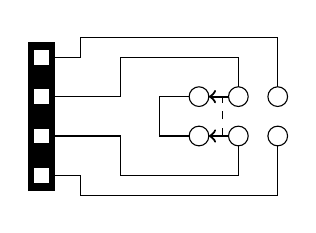
\begin{tikzpicture}[scale=.5]
		\draw [line width=10] (1,.6)--(1,4.4);
		\draw (6,3.25) -- (6,4) -- (3,4) -- (3,3) -- (1,3);
		\draw (6,1.75) -- (6,1) -- (3,1) -- (3,2) -- (1,2);
		\draw (7,3.25) -- (7,4.5) -- (2,4.5) -- (2,4) -- (1,4);
		\draw (7,1.75) -- (7,.5) -- (2,.5) -- (2,1) -- (1,1);
		\foreach \y in {1, 2, 3, 4} {
			\foreach \x in {1} {
				\draw [fill=white] (\x-.2,\y-.2) -- (\x-.2,\y+.2) -- (\x+.2,\y+.2) -- (\x+.2,\y-.2) -- cycle;
			}
		}
		\foreach \x in {5, 6, 7} {
			\foreach \y in {2, 3} {
				\draw (\x,\y) circle (.25);
			}
		}
		\draw [thick, ->] (5.75,2) -- (5.25,2);
		\draw [thick, ->] (5.75,3) -- (5.25,3);
		\draw [dashed]    (5.6,2) -- (5.6, 3);
		\draw (4.75,2) -- (4,2) -- (4,3) -- (4.75, 3);
	\end{tikzpicture}
\end{center}
